%%=============================================================================
%% Methodologie
%%=============================================================================

\chapter{\IfLanguageName{dutch}{Methodologie}{Methodology}}%
\label{ch:methodologie}

%% TODO: In dit hoofdstuk geef je een korte toelichting over hoe je te werk bent
%% gegaan. Verdeel je onderzoek in grote fasen, en licht in elke fase toe wat
%% de doelstelling was, welke deliverables daaruit gekomen zijn, en welke
%% onderzoeksmethoden je daarbij toegepast hebt. Verantwoord waarom je
%% op deze manier te werk gegaan bent.
%% 
%% Voorbeelden van zulke fasen zijn: literatuurstudie, opstellen van een
%% requirements-analyse, opstellen long-list (bij vergelijkende studie),
%% selectie van geschikte tools (bij vergelijkende studie, "short-list"),
%% opzetten testopstelling/PoC, uitvoeren testen en verzamelen
%% van resultaten, analyse van resultaten, ...
%%
%% !!!!! LET OP !!!!! 
%% Het is uitdrukkelijk NIET de bedoeling dat je het grootste deel van de corpus 
%% van je bachelorproef in dit hoofdstuk verwerkt! Dit hoofdstuk is eerder een 
%% kort overzicht van je plan van aanpak.
%% Maak voor elke fase (behalve het literatuuronderzoek) een NIEUW HOOFDSTUK aan
%% en geef het een gepaste titel.

\subsection{Fase 1: App-ontwikkeling en modelselectie}
In de eerste fase van het onderzoek ligt de focus op het ontwikkelen van een applicatie die de camera kan gebruiken voor het verwerken van gebaren. De applicatie zal fungeren als de interface tussen de gebruiker en het model, en zorgt ervoor dat de camera-beeldgegevens van de gebruiker kunnen worden vastgelegd en verwerkt.

Daarnaast wordt er gezocht naar een geschikt deep learning-model dat in staat is om gebarentaal te herkennen en om te zetten in tekst. Dit model zal worden gekozen op basis van de literatuurstudie en de beschikbaarheid van bestaande, pre-getrainde modellen. Er zal een focus liggen op de effectiviteit van het model in termen van nauwkeurigheid en snelheid, zodat het geschikt is voor gebruik in real-time toepassingen.

Deze fase zal een periode van 2 weken innemen, waarin het ontwikkelen van de app en het selecteren van een geschikt model centraal staan, evenals het uitvoeren van initiële tests met het model \ref{fig:flowchart_tijd}.

\subsection{Fase 2: Modeloptimalisatie}
In de tweede fase van het onderzoek zal het gekozen model geoptimaliseerd worden om efficiënter te werken. 
Dit gebeurt door parameters en architectuurcomponenten, zoals het aantal en type lagen, te analyseren en indien nodig aan te passen. 
De optimalisatie is gericht op het verbeteren van de snelheid en efficiëntie, zodat het model beter geschikt is voor gebruik op mobiele apparaten.

Daarnaast worden technieken zoals pruning en quantization onderzocht om het model geschikt te maken voor de beperkte rekenkracht van mobiele apparaten. 
Deze technieken helpen bij het verkleinen van het model en verbeteren de prestaties zonder concessies te doen aan de nauwkeurigheid.

Voordat het model wordt geïntegreerd in de applicatie, zal het eerst worden getest in een Python-notebook. 
Dit stelt ons in staat om de basisfunctionaliteit en nauwkeurigheid van het model te evalueren zonder de complexiteit van de mobiele implementatie. 
Door eerst tests in de notebook uit te voeren, kunnen we een solide basis leggen en ervoor zorgen dat de performance voldoet aan de vereisten.

Op basis van de testresultaten kunnen eventuele aanpassingen worden doorgevoerd voordat het model verder geoptimaliseerd wordt en later in de app wordt geïntegreerd.

Deze fase zal 6 weken duren, waarin zowel de modeloptimalisatie als de testen plaatsvinden, inclusief de aanpassingen op basis van de testresultaten en performanceverbeteringen \ref{fig:flowchart_tijd}.

\subsection{Fase 3: Model implementeren in de app}
In deze fase wordt het geoptimaliseerde model geïntegreerd in de applicatie. 
Dit is een cruciale stap, aangezien het model nu operationeel moet worden in een echte applicatieomgeving op een mobiel apparaat.

De eerste stap is het exporteren van het model naar een geschikt formaat, zoals TensorFlow Lite of ONNX, zodat het gemakkelijk in de app kan worden geladen. 
Vervolgens wordt het model geïmplementeerd in de applicatiecode en getest op de app-omgeving.

De applicatie wordt geconfigureerd zodat de camera-feed van de gebruiker wordt gekoppeld aan het model voor real-time gebarentaalherkenning. 

Deze fase is essentieel voor het testen van de interactie tussen de applicatie, de camera, en het model, en zal helpen bij het identificeren van eventuele problemen met de integratie.

Deze fase zal 4 weken duren, waarin de integratie van het model in de app en het testen van de interacties plaatsvindt \ref{fig:flowchart_tijd}.

\subsection{Fase 4: Evaluatie \& Validatie}
In de laatste fase van het onderzoek wordt het model geëvalueerd en gevalideerd. 
Dit gebeurt door middel van tests op een aparte dataset om de nauwkeurigheid en real-time prestaties te meten. 
De focus ligt hierbij op het testen van het model op ongeziene data om de generaliseerbaarheid en robuustheid van het model te waarborgen.

Daarnaast zal het model worden getest in real-time omstandigheden om te beoordelen hoe goed het functioneert bij het verwerken van live camera-invoer. 
Eventuele tekortkomingen in het model worden geanalyseerd en indien nodig verbeterd.

Deze fase zal 2 weken duren, waarin de tests op een aparte dataset en de real-time validatie plaatsvinden, gevolgd door het analyseren van de testresultaten en het doorvoeren van verbeteringen indien nodig \ref{fig:flowchart_tijd}.

\begin{figure}[h!]
  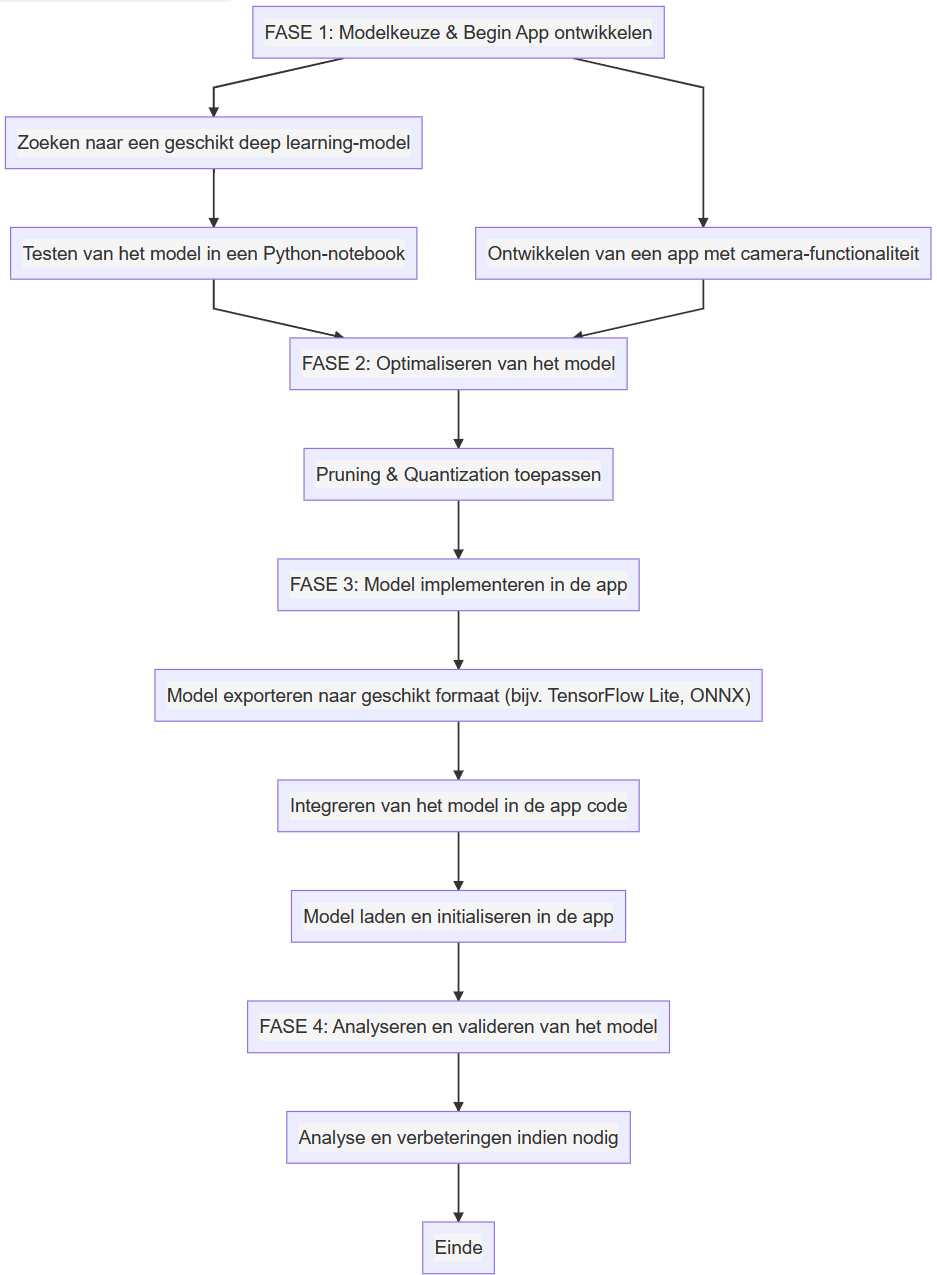
\includegraphics[width=0.5\textwidth]{../graphics/flowchart.png}
  \caption{Tijdlijn van het onderzoek}
  \label{fig:flowchart_tijd}
\end{figure}
